\documentclass[tikz]{standalone}
\usepackage{tikz}
\usepackage{alphalph}
\usetikzlibrary{positioning, graphs}
\usetikzlibrary{graphs.standard}
\usetikzlibrary{arrows.meta}
\begin{document}
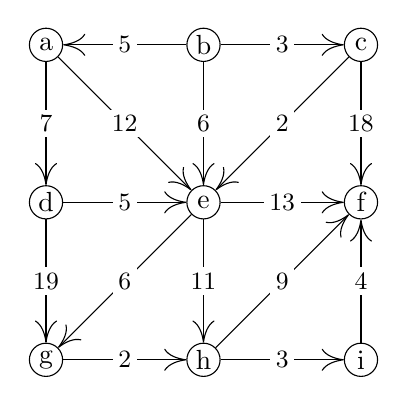
\begin{tikzpicture}
\begin{scope}
		[vertex/.style={draw,circle,inner sep = 0em, minimum size = 1.2em},
		 edgelabel/.style = {fill = white, inner sep = 0.2em, font=\small}]
		\node[vertex] (a) at (0, 0) {a};
		\node[vertex] (b) at (2, 0) {b};
		\node[vertex] (c) at (4, 0) {c};
		\node[vertex] (d) at (0,-2) {d};
		\node[vertex] (e) at (2,-2) {e};
		\node[vertex] (f) at (4,-2) {f};
		\node[vertex] (g) at (0,-4) {g};
		\node[vertex] (h) at (2,-4) {h};
		\node[vertex] (i) at (4,-4) {i};
		
		\draw[-{>[length=8, width=8]}] (a) to node[edgelabel] {$7$} (d);
		\draw[-{>[length=8, width=8]}] (a) to node[edgelabel] {$12$} (e);
		\draw[-{>[length=8, width=8]}] (b) to node[edgelabel] {$5$} (a);
		\draw[-{>[length=8, width=8]}] (b) to node[edgelabel] {$3$} (c);
		\draw[-{>[length=8, width=8]}] (b) to node[edgelabel] {$6$} (e);
		\draw[-{>[length=8, width=8]}] (c) to node[edgelabel] {$2$} (e);
		\draw[-{>[length=8, width=8]}] (c) to node[edgelabel] {$18$} (f);
		\draw[-{>[length=8, width=8]}] (d) to node[edgelabel] {$5$} (e);
		\draw[-{>[length=8, width=8]}] (d) to node[edgelabel] {$19$} (g);
		\draw[-{>[length=8, width=8]}] (e) to node[edgelabel] {$6$} (g);
		\draw[-{>[length=8, width=8]}] (e) to node[edgelabel] {$11$} (h);
		\draw[-{>[length=8, width=8]}] (e) to node[edgelabel] {$13$} (f);
		\draw[-{>[length=8, width=8]}] (g) to node[edgelabel] {$2$} (h);
		\draw[-{>[length=8, width=8]}] (h) to node[edgelabel] {$9$} (f);
		\draw[-{>[length=8, width=8]}] (h) to node[edgelabel] {$3$} (i);
		\draw[-{>[length=8, width=8]}] (i) to node[edgelabel] {$4$} (f);
		
\end{scope}
\end{tikzpicture}
\end{document}